
\subsection{Kernel Generation}
\begin{frame}{Kernel Generation}
  \begin{columns}[c]
    \column{.54\textwidth}
    \only<1>{%
        \begin{block}{Hits}
        \begin{itemize}
            \item Hits lie on the 26 planes
            \item Tracks come from PVs and SVs
            \item For simplicity, only 3 tracks shown
            \item Hits are sorted in $r$ (distance from LHC beam)
        \end{itemize}
        \end{block}
    }
    \only<2>{%
        \begin{block}{Grid}
        \begin{itemize}
            \item Make a 3D grid of voxels (2D shown)
            \item \textcolor{brickred}{Note: only $z$ will be fully calculated and stored}
        \end{itemize}
        \end{block}
    }
    \only<3-5>{%
        \begin{block}{Prototrack}
        \begin{itemize}
            \item Start with maximum $r$
            \item Find triplet with $\chi^2<10$
            \item Mark ``used'' all other hits within $\chi^2<9$
            \item \textcolor{brickred}{Note: triplet is stored}
        \end{itemize}
        \end{block}

        \begin{block}{Kernel}
        \begin{itemize}
            \item Fill in each voxel center with gaussian PDF
            \item PDF is combined for each prototrack
        \end{itemize}
        \end{block}

    }
    \only<6>{%
        \begin{block}{Kernel}
        \begin{itemize}
            \item Highest PDF density at vertices
            \item Stores $z$ histogram with maximum PDF values
        \end{itemize}
        \end{block}

        \begin{block}{Details}
        \begin{itemize} \color{brickred}
            \item $x$-$y$ grid initially very coarse
            \item Search performed on maximum $x$-$y$ grid cell using stored triplets to recalculate PDF
        \end{itemize}
        \end{block}
    }

    \column{.46\textwidth}
    \begin{tikzpicture}
        [hit/.style={inner sep=2pt, fill, circle, black!80!red},
        simitrack/.style={shorten >= -6cm, shorten <= -6cm, opacity=.2, line width=.1cm,
            preaction={draw, line width=.3cm, opacity=.2},
            preaction={draw, line width=.5cm, opacity=.2}},
        bluesimitrack/.style={thick, blue,
            preaction={shorten >= -6cm, shorten <= -6cm, draw, opacity=.2, line width=.1cm,
                preaction={draw, blue, line width=.3cm, opacity=.2},
                preaction={draw, blue, line width=.5cm, opacity=.2}}}
        ]

        \node at (2,-3) [below] {$z$ axis (along the beam)};
        \node at (-1, 0) [left] {$x$};

        \clip (-1,-3) rectangle (5,3);

        \begin{scope}[xscale=.65, xshift=-.6cm]

        % def f(name, slope, factor):
        %     v = np.arange(1,9)
        %     vv = (v-.5)*slope + .05*np.sin(v*factor)
        %     q = np.linspace(.5, 8, 400)
        %     qq = (q-.5)*slope + .05*np.sin(q*factor)
        %     print(f'% {name} slope={slope} factor={factor}')
        %     for a,b in zip(v,vv):
        %         print(f'\coordinate ({name}{a}) at ({a}, {b:.3});')
        %     print()
        %     return q, qq, v, vv


        % (v-.5)*slope + .05*np.sin(v*factor)
        % A slope=0.4 factor=-5
        \coordinate (A1) at (1, 0.248);
        \coordinate (A2) at (2, 0.627);
        \coordinate (A3) at (3, 0.967);
        \coordinate (A4) at (4, 1.35);
        \coordinate (A5) at (5, 1.81);
        \coordinate (A6) at (6, 2.25);
        \coordinate (A7) at (7, 2.62);

        % B slope=0.06 factor=6
        \coordinate (B1) at (1, 0.016);
        \coordinate (B2) at (2, 0.0632);
        \coordinate (B3) at (3, 0.112);
        \coordinate (B4) at (4, 0.165);
        \coordinate (B5) at (5, 0.221);
        \coordinate (B6) at (6, 0.28);
        \coordinate (B7) at (7, 0.344);
        \coordinate (B8) at (8, 0.412);

        % C slope=-0.35 factor=7
        \coordinate (C1) at (1, -0.142);
        \coordinate (C2) at (2, -0.475);
        \coordinate (C3) at (3, -0.833);
        \coordinate (C4) at (4, -1.21);
        \coordinate (C5) at (5, -1.6);
        \coordinate (C6) at (6, -1.97);
        \coordinate (C7) at (7, -2.32);

        \only<1>{%
        \foreach \x in {0,...,9}{%
            \draw [ultra thick, yellow!80!black] (\x, -3) -- (\x,3);
        }
        }
        \end{scope}

        \only<2->{%
        \draw[step=.5, gray, very thin, use as bounding box] (-1,-3) grid (5,3);
        }

        \only<3>{%
            \draw [bluesimitrack] (A5) -- (A7) ;
        } \only<4->{%
            \draw [simitrack] (A5) -- (A7) ;
        }

        \only<4>{%
            \draw [bluesimitrack] (B6) -- (B8) ;
        } \only<5->{%
            \draw [simitrack] (B6) -- (B8) ;
        }

        \only<5>{%
            \draw [bluesimitrack] (C5) -- (C7) ;
        } \only<6->{%
            \draw [simitrack] (C5) -- (C7) ;
        }

        \draw [fill,green!60!black] (0,0) circle (.065) node [left] {PV};

        \only<0-2>{%
        \node [hit] at (A1) {};
        \node [hit] at (A2) {};
        \node [hit] at (A3) {};
        \node [hit] at (A4) {};
        }\only<3->{%
        \node [hit, red] at (A1) {};
        \node [hit, red] at (A2) {};
        \node [hit, red] at (A3) {};
        \node [hit, red] at (A4) {};
        }

        \only<0-2>{%
        \node [hit] at (A5) {};
        \node [hit] at (A6) {};
        \node [hit] at (A7) {};
        } \only<3>{%
        \node [hit, blue] at (A5) {};
        \node [hit, blue] at (A6) {};
        \node [hit, blue] at (A7) {};
        } \only<4->{%
        \node [hit, red] at (A5) {};
        \node [hit, red] at (A6) {};
        \node [hit, red] at (A7) {};
        }

        \only<0-3>{%
        \node [hit] at (B1) {};
        \node [hit] at (B2) {};
        \node [hit] at (B3) {};
        \node [hit] at (B4) {};
        \node [hit] at (B5) {};
        \node [hit] at (C1) {};
        } \only<4->{%
        \node [hit, red] at (B1) {};
        \node [hit, red] at (B2) {};
        \node [hit, red] at (B3) {};
        \node [hit, red] at (B4) {};
        \node [hit, red] at (B5) {};
        \node [hit, red] at (C1) {};
        }

        \only<0-3>{%
        \node [hit] at (B6) {};
        \node [hit] at (B7) {};
        \node [hit] at (B8) {};
        } \only<4>{%
        \node [hit, blue] at (B6) {};
        \node [hit, blue] at (B7) {};
        \node [hit, blue] at (B8) {};
        }\only<5->{%
        \node [hit, red] at (B6) {};
        \node [hit, red] at (B7) {};
        \node [hit, red] at (B8) {};
        }

        \only<0-4>{%
        \node [hit] at (C2) {};
        \node [hit] at (C3) {};
        \node [hit] at (C4) {};
        } \only<5->{%
        \node [hit, red] at (C2) {};
        \node [hit, red] at (C3) {};
        \node [hit, red] at (C4) {};
        }

        \only<0-4>{%
        \node [hit] at (C5) {};
        \node [hit] at (C6) {};
        \node [hit] at (C7) {};
        } \only<5>{%
        \node [hit, blue] at (C5) {};
        \node [hit, blue] at (C6) {};
        \node [hit, blue] at (C7) {};
        } \only<6->{%
        \node [hit, red] at (C5) {};
        \node [hit, red] at (C6) {};
        \node [hit, red] at (C7) {};
        }

    \end{tikzpicture}

    \end{columns}
\end{frame}


% Part 3: HENRY
\subsection{Example of z KDE histogram}
\begin{frame}{Example of z KDE histogram}
\begin{center}
    \includegraphics[width=\textwidth, trim=50 30 50 30]{images/kernel_and_pvs.pdf}
\end{center}
\begin{columns}[t]
    \column{.55\textwidth}
    \begin{block}{Human learning}
    \begin{itemize}
        \item Peaks generally correspond to PVs and SVs
    \end{itemize}
    \end{block}

    \column{.45\textwidth}
    \begin{block}{Challenges}
    \begin{itemize}
        \item Vertex may be offset from peak
        \item Vertices interact
    \end{itemize}
    \end{block}
\end{columns}
\end{frame}


% Zoom in

% rui add a target histogram
\subsection{Distribution of Target}
\begin{frame}{Target distribution}
\begin{columns}[c]
    \column{.5\textwidth}
    \begin{block}{Build target distribution}
      \begin{itemize}
          \item real PV position as the mean of Gaussian distribution
          \item $\sigma $(standard deviation) is 100 $\mu$m
          \item calculate the cdf of each bin around of the mean, within $\pm$ 3 bins ($\pm$ 300 $\mu$m )
      \end{itemize}
    \end{block}
    \begin{center}
            \includegraphics[width=1\textwidth,height=0.45\textwidth,trim=18 0 18 0]{images/T_1_12.png}

        \end{center}
    \column{.5\textwidth}
      \begin{center}
    \includegraphics[width=1\textwidth,height=0.45\textwidth, trim=18 0 18 0]{images/T_2_12.png}

    \includegraphics[width=1\textwidth,height=0.45\textwidth, trim=18 0 18 0]{images/T_2_25.png}
  \end{center}
  \end{columns}
\end{frame}


\subsection{Preliminary study}
\begin{frame}{Preliminary study}
\begin{columns}[c]
    \column{.5\textwidth}
    \begin{block}{Preliminary study}
      \begin{itemize}
          \item 2, 3, and 4 convolutional layers
          \item Symmetric cost function to be described
          \item Discovered ``low multiplicity'' PVs are counted as false positives
      \end{itemize}
    \end{block}
    \column{.5\textwidth}
    \begin{block}{Current work}
      \begin{itemize}
          \item Add masking to not count discovered ``low multiplicity'' as false positives
          \item Asymmetric cost function to control trade-offs between efficiency  and false positive rates
      \end{itemize}
    \end{block}
  \end{columns}
\end{frame}



% Part 5: RUI
\subsection{Neural network architecture}
\begin{frame}{Neural network architecture with two convolutional layers}
    \begin{center}
      \includegraphics[width=0.75\linewidth, trim=0 30 0 0]{images/CNN_2.png}
   \end{center}
   \begin{itemize}
       \item Activation function for hidden layers: Leaky ReLu
       \item Activation function for output layer: Sigmoid
   \end{itemize}
\end{frame}
\begin{frame}{Activation function}
   \begin{columns}[c]
   % TODO: Swap
        \column{.5\textwidth}
        \begin{center}
            \includegraphics[width=0.8\textwidth]{images/LeakyRelu.png}

            Activation function for hidden layers
        \end{center}

        \column{.5\textwidth}
        \begin{center}
            \includegraphics[width=0.8\textwidth]{images/Sigmoid.png}

            Activation function for output layer
        \end{center}
  \end{columns}
\end{frame}


% Part 4: MDS
\subsection{Cost Function}
\begin{frame}{Cost Function}
  \begin{columns}[c]
    \column{0.45\textwidth}
    \begin{block}{Approach}
      \begin{itemize}
         \item
           Cost function should be similar to Cross-Entropy for $ y \to 0 $,
           $ y \to 1 $;
             $ \color{brickred} \textrm{cost} = - \big (y \ln \hat{y} + (1-y) \ln (1 - \hat{y}) \big )  $
         \item
          Should be symmetric with respect to  $ r = ( \hat y/y  )$ \& $ 1/r $
     \end{itemize}
    \end{block}
    \begin{block}{Sum Over Bins}
      \begin{equation}
        \color{brickred}
        r_i \equiv (\hat{y_i} + \epsilon)/ (y_i + \epsilon)
      \end{equation}
      \vspace{-.9em}
      \begin{equation}
        \color{brickred}
        z_i \equiv \frac{2 \, r_i }{r_i + 1/r_i}
      \end{equation}
      \vspace{-.4em}
      \begin{equation}
        \color{brickred}
        \textrm{our cost} = \sum_{\textrm{bins}} {- \ln{z_i}}
      \end{equation}
      \vspace{-.7em}
    \end{block}
    \column{0.6\textwidth}
      \centering
      \includegraphics[width=1.0\linewidth]{images/CostPlot.png}
      \end{columns}
\end{frame}
